\subsection{The edge of the drift volume: a field fringe at the unpassivated sides}\label{sec:edge}
\sectionstate{partial}{\texttt{rerun/paper1\_figs/README.md} (edge study, pass 1, 2026-10-31: \texttt{edge\_study.py},
\texttt{edge\_angles.py}); figure \texttt{edge\_turnon}}
\intent{Dylan 2026-11-02: expand the edge study; keep it separate from the bow (different mechanisms). What happens near the
chamber sides, measured three independent ways with the same depth, why it occurs only on the two sides without
passivation (\cref{sec:design_choices}), and why it sets the 30\,mm fiducial for angles but not for efficiency.}

\textbf{Three signals, one depth.} Within 20--30\,mm of the two $x$ sides ($x=0$ and $398.6$\,mm, no passivation):
(i) the X angle is biased, $\tan_\mathrm{fit}-\tan_\mathrm{ref}$ up to 0.1--0.36 within 5--20\,mm of a side and below 0.01 by
30\,mm, with opposite signs on the two sides on chambers A, C and E: the drift lines converge inwards, so charge released
near the cathode lands further inside than it started; (ii) the drift column is longer (A up to $+1.1$\,\textmu s at
5--10\,mm; B $+0.17/+0.48$\,\textmu s), with more charge and more strips: the edge strips collect electrons from outside
the strip area, over longer paths; (iii) the efficiency reaches its plateau by 10--20\,mm on the $x$ sides, by ${\sim}5$\,mm
on the passivated $y$ sides. These use no track model (ii), the reference (i, iii), or both.
\textbf{Not the bow.} The bow predicts the edge column \emph{shorter} (mesh nearer the cathode at the rim, $-45$ to
$-64$\,ns), the fringe makes it longer; measured edge shifts $-4/{+26}/{+78}/{+27}/{-115}$\,ns (B/A/E/C/D) are the sum.
\textbf{The fiducial.} The passivated $y$ sides are sharp for efficiency but not for angles: a 10--30\,mm $y$ band keeps
full efficiency while its Y-angle $s_{68}$ is 1.3--1.9$\times$ the interior's (A, B). So the ${\ge}30$\,mm interior
is the right fiducial for angles and positions; for efficiency alone 10\,mm from the $y$ sides would do (+9--10\,\%
tracks).
\begin{figure}[tbp]
  \centering
  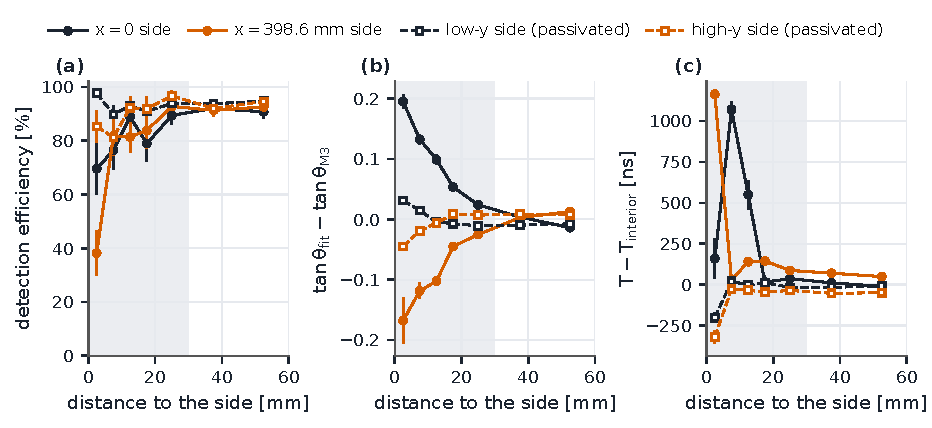
\includegraphics[width=\linewidth]{edge_turnon}
  \caption{Chamber~A near the chamber sides, against the distance of the reference ray (or the charge centroid in (c)) to the physical edge of the strip plane: (a) efficiency turn-on, (b) angle bias of the perpendicular view against the reference, (c) drift-column duration relative to the interior. Solid: the unpassivated $x$ sides; dashed: the passivated $y$ sides. Dotted vertical lines: where the passivation ends on the low-$y$ (18.0\,mm) and high-$y$ (18.7\,mm) side. Error bars: binomial in (a); $1.25\,s_{68}/\sqrt{n}$ in (b). In (b), bins in which fewer than 30\,\% of the rays are detected are not shown (the passivated band); in (c) there are no triggers with a charge centroid in the passivated band.}
  \label{fig:edge}
\end{figure}
\textbf{What the edges cost the headline.} The efficiency is quoted over the full active area (Dylan 2026-11-02);
against the interior it loses 0.8\,pt (production pick 91.5 vs 92.3\,\%) and 0.9\,pt single-track (94.8 vs 95.7\,\%),
all of it within 30\,mm of the unpassivated $x$ sides and within 8\,mm of the passivated $y$ sides. The angles and positions
are quoted in the interior.
